\documentclass[tikz]{standalone}

\usepackage{tikz}
\usetikzlibrary{positioning, arrows.meta, shapes, snakes, shadings}
\usepackage{amsmath,amssymb,amsthm,pgfplots}

%% Sky colors:
%\definecolor{col1}{RGB}{254,251,87}
%\definecolor{col2}{RGB}{193,86,98}
%\definecolor{col3}{RGB}{179,191,245}
%\definecolor{col4}{RGB}{117,249,240}
%\definecolor{col5}{RGB}{234,138,51}
%\definecolor{col6}{RGB}{158,93,202}
%\definecolor{col7}{RGB}{148,110,107}
%\definecolor{col8}{RGB}{243,201,133}
%\definecolor{col9}{RGB}{240,254,238}
%\definecolor{col10}{RGB}{175,227,71}
%\definecolor{col11}{RGB}{93,197,229}
%\definecolor{col12}{RGB}{231,63,240}
%\definecolor{col13}{RGB}{226,48,34}
%\definecolor{col14}{RGB}{237,127,197}
%\definecolor{col15}{RGB}{79,130,131}
%\definecolor{col16}{RGB}{175,53,245}
%\definecolor{col17}{RGB}{73,169,246}
%\definecolor{col18}{RGB}{234,53,132}
%\definecolor{col19}{RGB}{148,248,184}
%\definecolor{col20}{RGB}{77,109,246}
%\definecolor{col21}{RGB}{234,253,173}
%\definecolor{col22}{RGB}{246,198,236}
%\definecolor{col23}{RGB}{93,136,65}
%\definecolor{col24}{RGB}{116,249,115}

%% Kelly:
\definecolor{col1}{RGB}{242,243,244}
\definecolor{col2}{RGB}{175,35,55}
\definecolor{col3}{RGB}{236,195,66}
\definecolor{col4}{RGB}{41,103,160}
\definecolor{col5}{RGB}{47,60,40}
\definecolor{col6}{RGB}{150,180,55}
\definecolor{col7}{RGB}{218,147,171}
\definecolor{col8}{RGB}{229,137,50}
\definecolor{col9}{RGB}{128,89,143}
\definecolor{col10}{RGB}{126,51,31}
\definecolor{col11}{RGB}{59,133,90}
\definecolor{col12}{RGB}{192,178,134}
%\definecolor{col13}{RGB}{169,201,237}
%\definecolor{col14}{RGB}{236,151,127}
%\definecolor{col15}{RGB}{132,132,130}
%\definecolor{col16}{RGB}{96,70,40}
%\definecolor{col17}{RGB}{210,96,52}
%\definecolor{col18}{RGB}{166,76,107}
%\definecolor{col19}{RGB}{219,210,69}
%\definecolor{col20}{RGB}{235,168,59}
%\definecolor{col21}{RGB}{93,80,146}
%\definecolor{col22}{RGB}{34,34,34}

\begin{document}

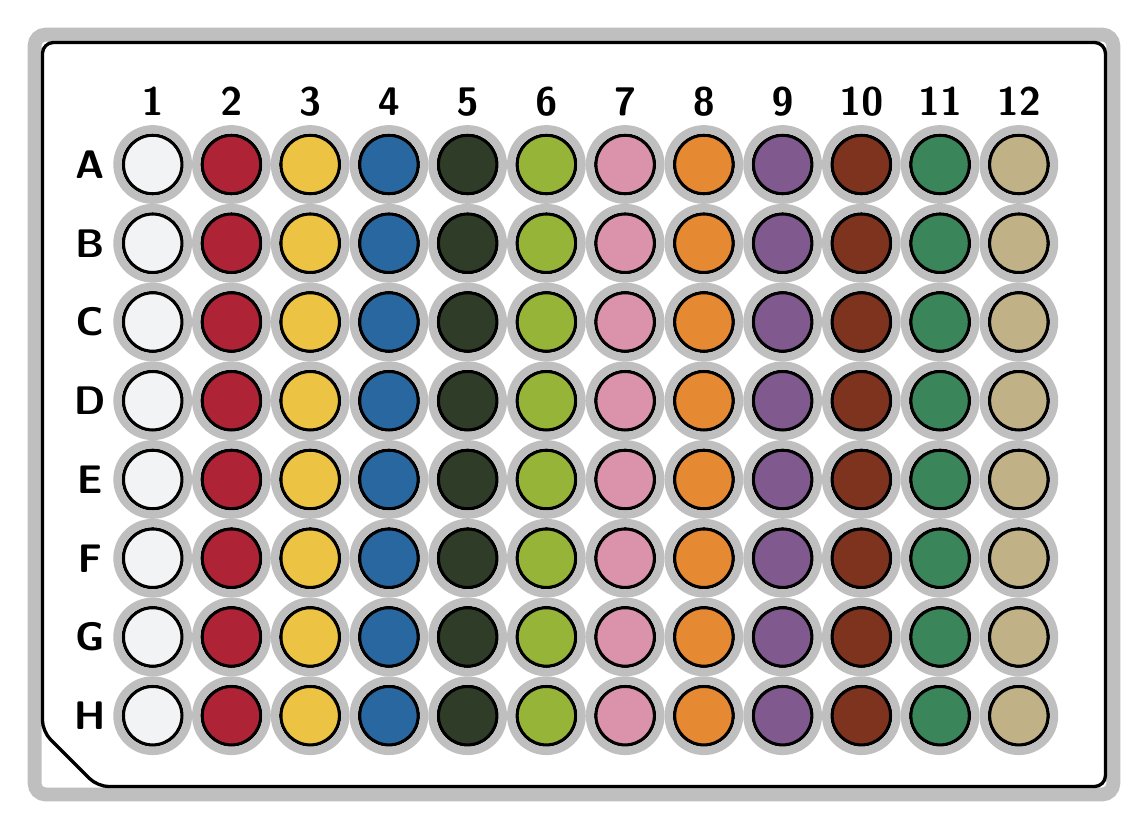
\begin{tikzpicture}
%    \draw[very thick] (0.75,0.25) -- (12.75,0.25) -- 
%                            (12.75,8.75) -- (0.25,8.75) --
%                            (0.25,0.75) --cycle;
    \draw[line width=5pt, lightgray, rounded corners] (-0.5,0) rectangle (13.2,9.65);
    \draw[very thick, rounded corners] (0.3,0.1) -- (13.1,0.1) -- (13.1,9.55) --
                                       (-0.4,9.55) -- (-0.4,0.8) --cycle;
    \foreach \i in {1,...,12} {
        \draw (\i, 8.8) node {\Large \sffamily \bfseries \i};
        \foreach \j in {1,...,8} {
            \draw (\i, \j) node[circle, inner sep=7.5pt, draw, very thick, fill=col\i] {};
            \draw (\i, \j) node[circle, inner sep=9pt, draw=lightgray, line width=3pt] {};
        }
    }
    \draw (.2, 8) node {\Large \sffamily \bfseries  A}
          (.2, 7) node {\Large \sffamily \bfseries  B}
          (.2, 6) node {\Large \sffamily \bfseries  C}
          (.2, 5) node {\Large \sffamily \bfseries  D}
          (.2, 4) node {\Large \sffamily \bfseries  E}
          (.2, 3) node {\Large \sffamily \bfseries  F}
          (.2, 2) node {\Large \sffamily \bfseries  G}
          (.2, 1) node {\Large \sffamily \bfseries  H};
\end{tikzpicture}   

\end{document}